\chapter{Virtualization: Containers, Part
2}\label{virtualization-containers-part-2}

REVIEW OF VIRTUAL MACHINES (TYPE 1 and TYPE2 HYPERVISORS)

\begin{figure}
\centering
\pandocbounded{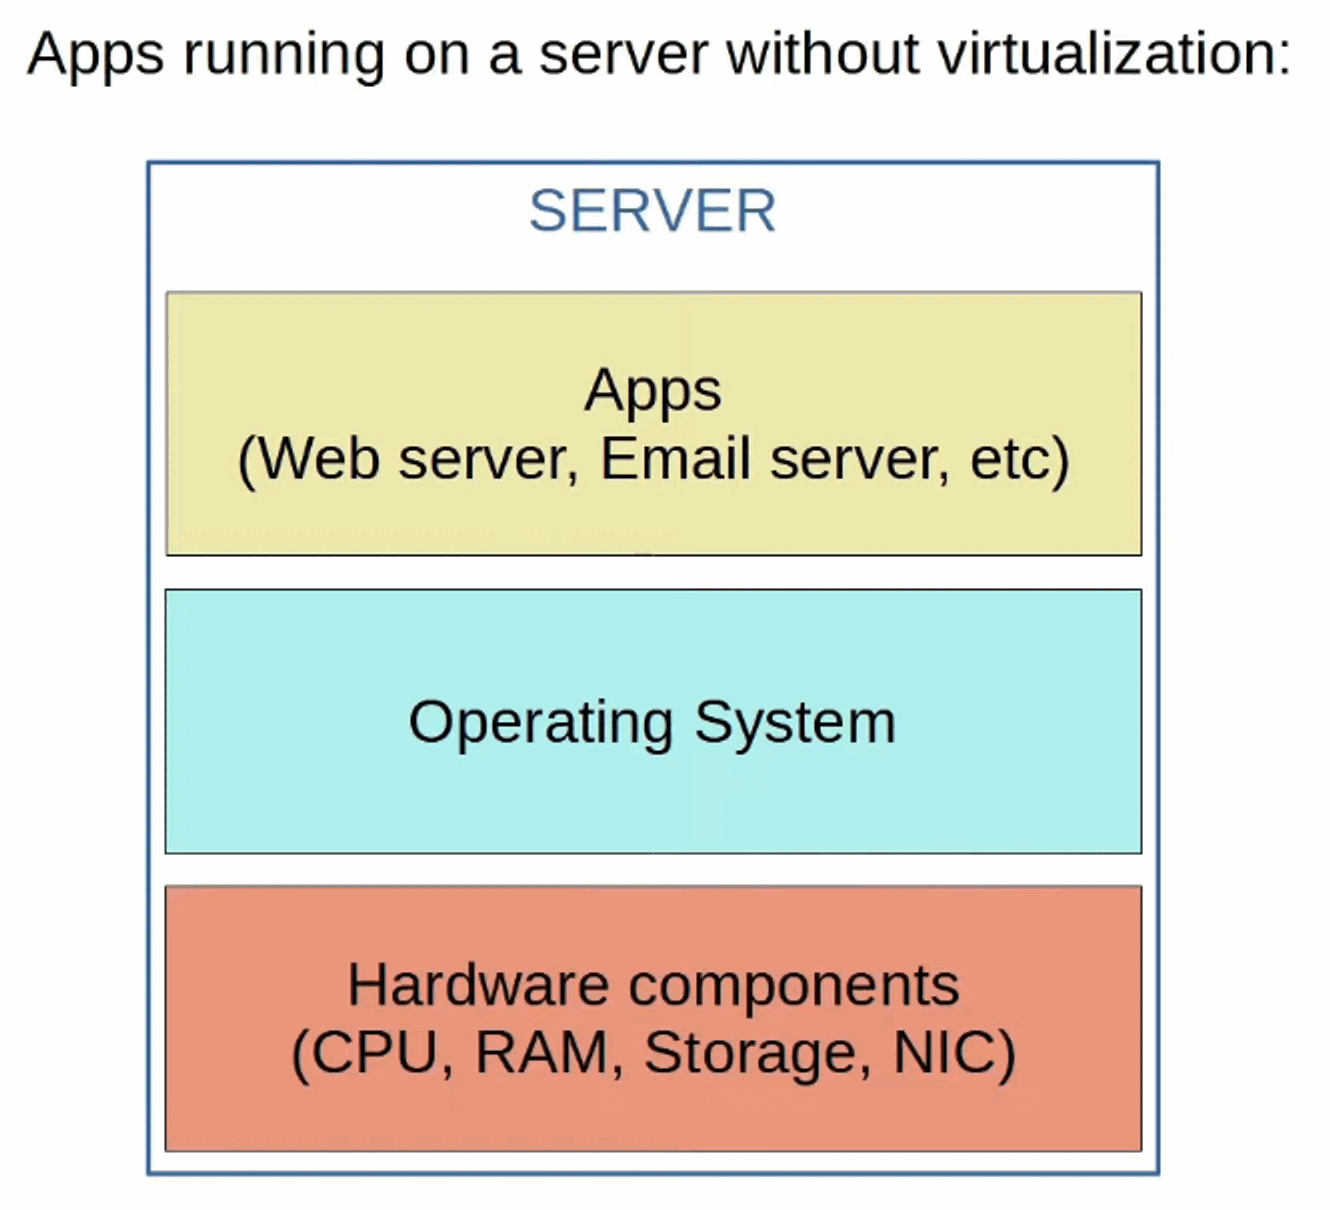
\includegraphics[keepaspectratio,alt={image}]{images/56-virtualization-containers/img-001.png}}
\end{figure}

\begin{figure}
\centering
\pandocbounded{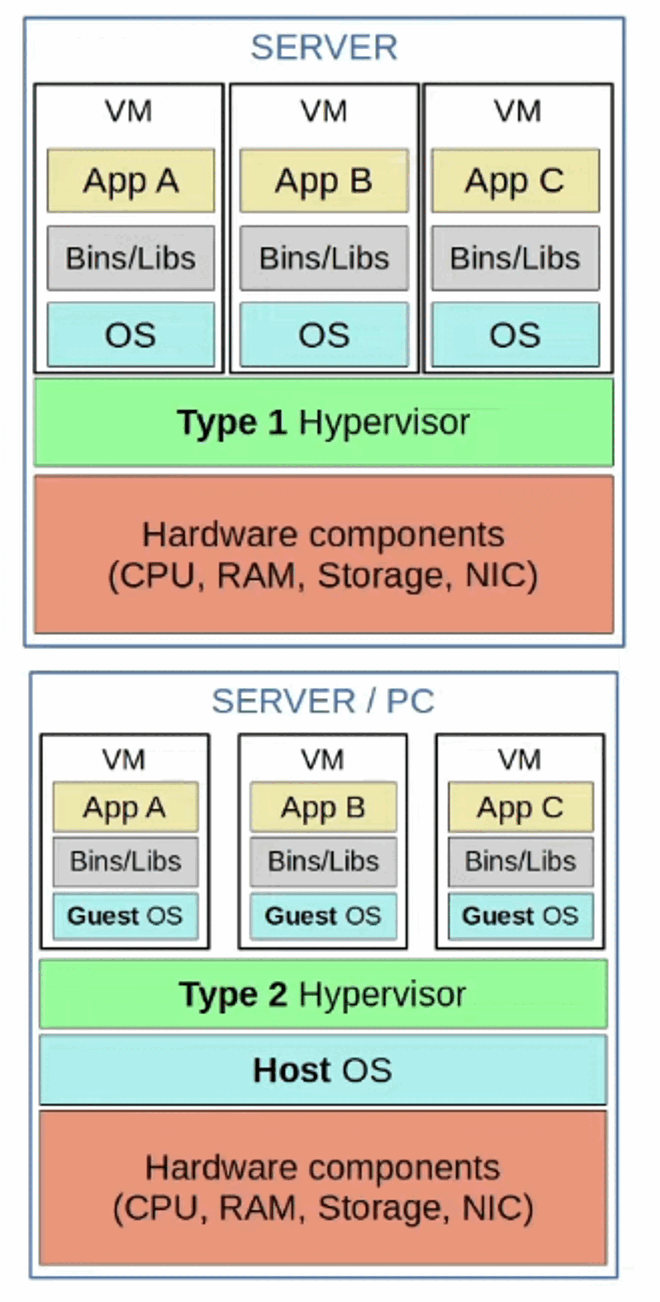
\includegraphics[keepaspectratio,alt={image}]{images/56-virtualization-containers/img-002.png}}
\end{figure}

\begin{itemize}
\tightlist
\item
  VIRTUAL MACHINES (VMs) allow multiple OS's to run on a single PHYISCAL
  SERVER
\item
  A HYPERVISOR is used to manage and allocate HARDWARE RESOURCES to each
  VM

  \begin{itemize}
  \tightlist
  \item
    TYPE 1 HYPERVISORS (aka NATIVE or BARE-METAL) run directly on top of
    HARDWARE
  \item
    TYPE 2 HYPERVISORS (aka HOSTED) run on top of a HOST OS (ie:
    WINDOWS)
  \end{itemize}
\item
  TYPE 1 HYPERVISORS are widely used in DATA CENTER ENVIRONMENTS
\item
  TYPE 2 HYPERVISORS are commonly used on personal DEVICES

  \begin{itemize}
  \tightlist
  \item
    Running a virtual network lab on your PC using Cisco Modeling Labs
    (CML)
  \end{itemize}
\item
  The OS in each VM can be the same or different (Windows, Linux, MacOS,
  etc)
\item
  \emph{Bins / Libs} are the SOFTWARE libraries / services needed by the
  Apps running in each VM
\item
  A VM allows it's app / apps to run in an ISOLATED environment,
  separate from the apps in other VMs.
\item
  VMs are easy to create, delete, move, etc.

  \begin{itemize}
  \tightlist
  \item
    A VM can be easily saved and moved between different physical
    SERVERS.
  \end{itemize}
\end{itemize}

\begin{figure}
\centering
\pandocbounded{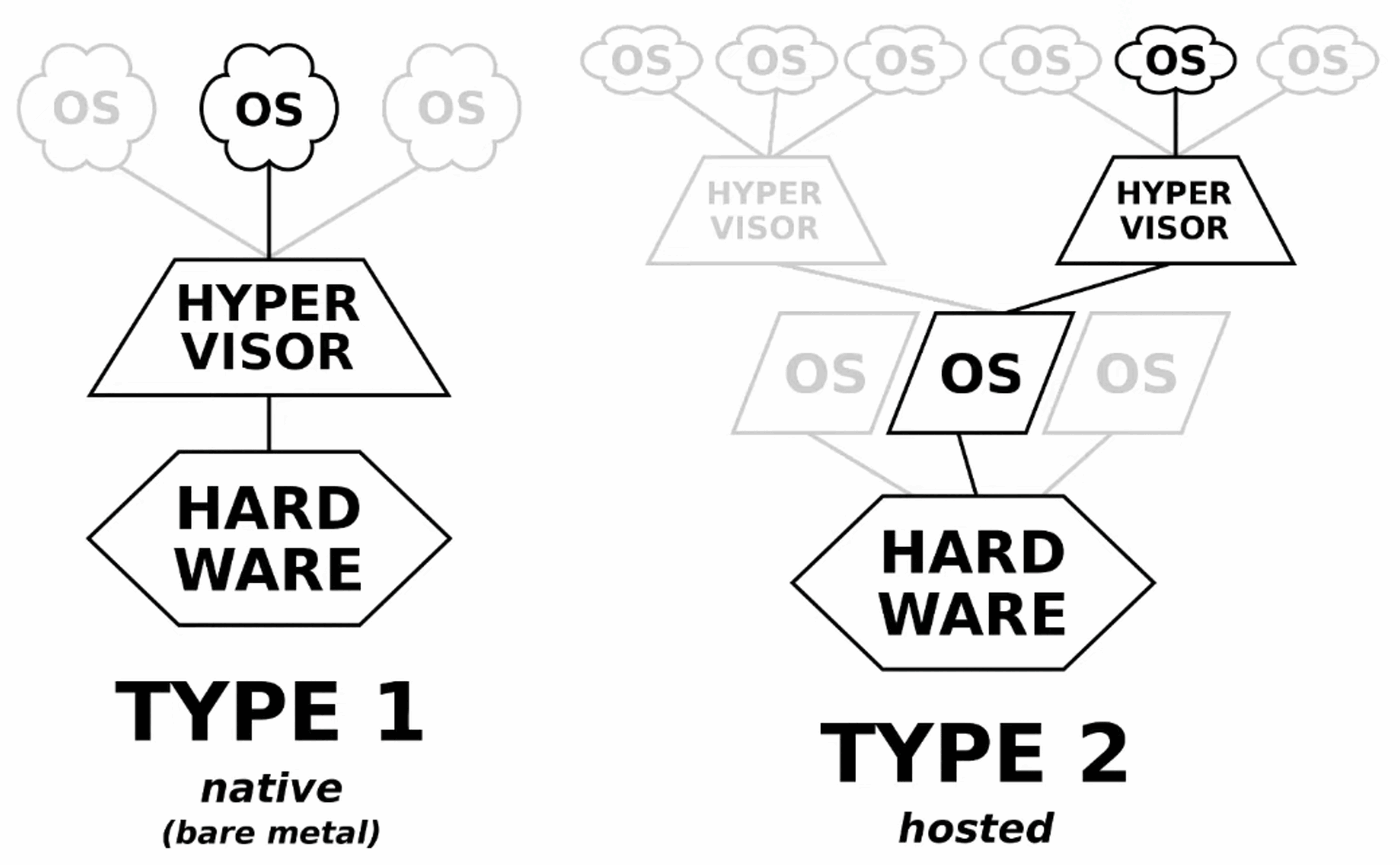
\includegraphics[keepaspectratio,alt={image}]{images/56-virtualization-containers/img-003.png}}
\end{figure}

\section{Containers}\label{containers}

\begin{figure}
\centering
\pandocbounded{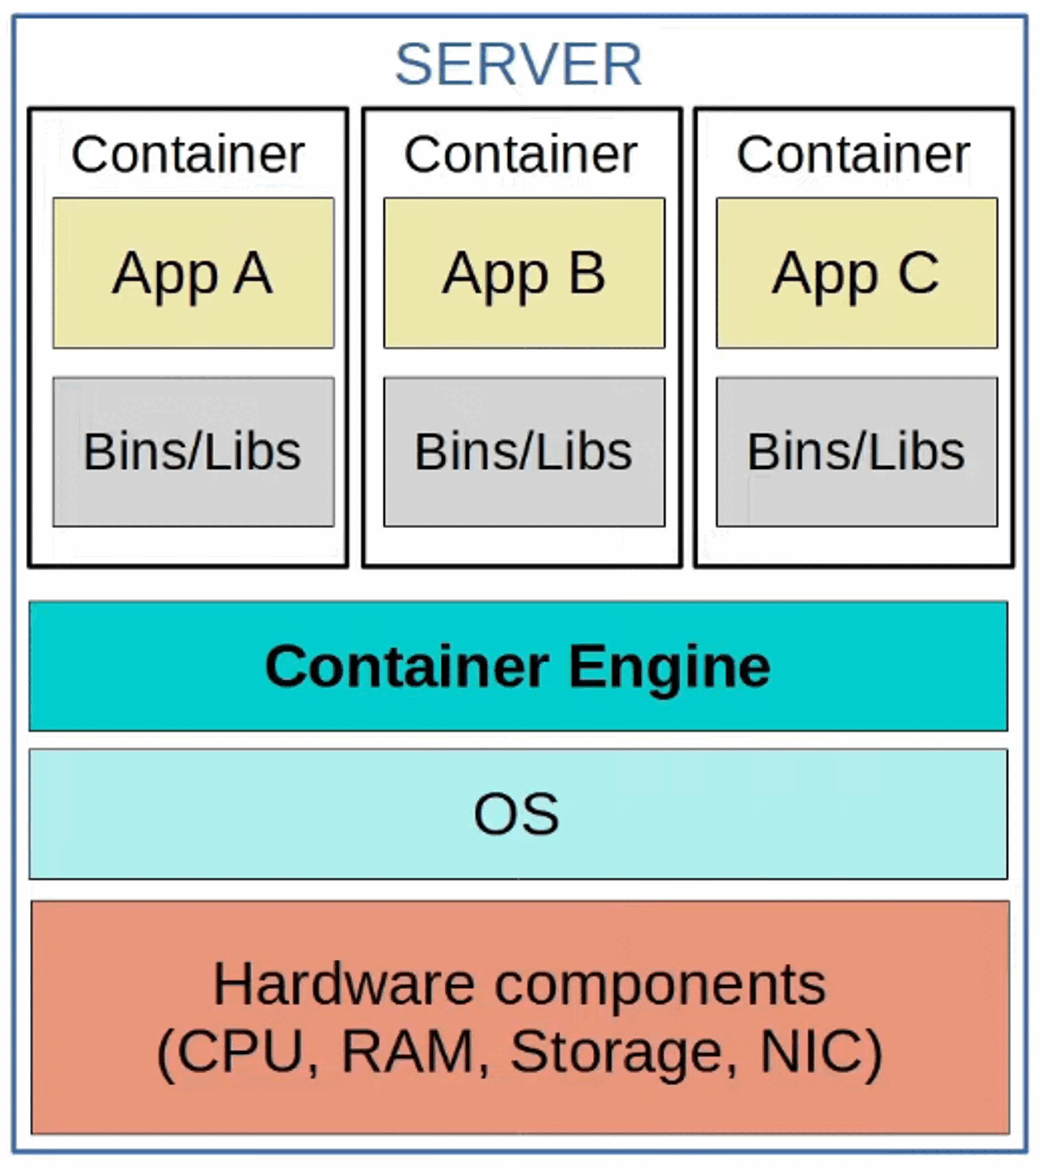
\includegraphics[keepaspectratio,alt={image}]{images/56-virtualization-containers/img-004.png}}
\end{figure}

\begin{itemize}
\tightlist
\item
  CONTAINERS are software packages that contain an APP and all
  dependencies (\emph{Bins/Libs} in the diagram) for the contained APP
  to run.

  \begin{itemize}
  \tightlist
  \item
    Multiple APPS can be run in a single CONTAINER, but this is not how
    CONTAINERS are usually used
  \end{itemize}
\item
  CONTAINERS run on a CONTAINER ENGINE (ie: DOCKER ENGINE)

  \begin{itemize}
  \tightlist
  \item
    The CONTAINER ENGINE is run on a HOST OS (usually LINUX)
  \end{itemize}
\item
  CONTAINERS are lightweight (small in size) and include only the
  dependencies required to run the specific APP
\item
  A CONTAINER ORCHESTRATOR is a software platform for automating the
  DEPLOYMENT, MANAGEMENT, SCALING, etc of CONTAINERS

  \begin{itemize}
  \tightlist
  \item
    KUBERNETES (originally design by Google) is the most popular
    CONTAINER ORCHESTRATOR
  \item
    DOCKER SWARM is DOCKER'S CONTAINER ORCHESTRATION tool
  \end{itemize}
\item
  In small numbers, MANUAL operation is possible, but large-scale
  systems (ie: with Microservices) can require THOUSANDS of CONTAINERS
\end{itemize}

\begin{figure}
\centering
\pandocbounded{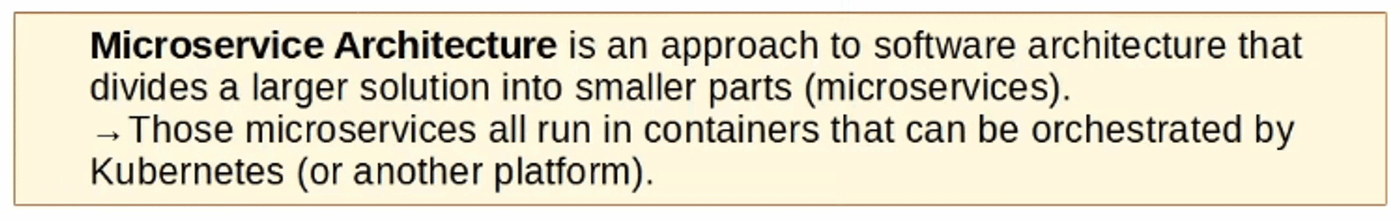
\includegraphics[keepaspectratio,alt={image}]{images/56-virtualization-containers/img-005.png}}
\end{figure}

VIRTUAL MACHINES vs.~CONTAINERS

\begin{figure}
\centering
\pandocbounded{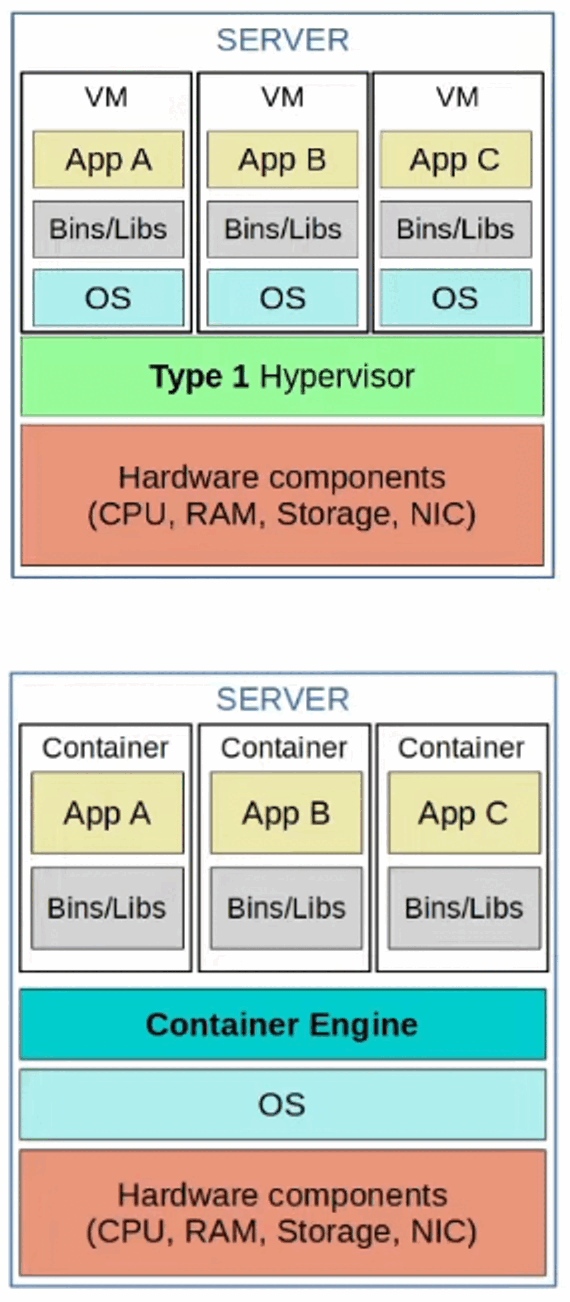
\includegraphics[keepaspectratio,alt={image}]{images/56-virtualization-containers/img-006.png}}
\end{figure}

\begin{itemize}
\item
  VMs can TAKE MINUTES to boot up as each VM runs it's own OS
\item
  CONTAINERS can boot up in milliseconds
\item
  VMs take MORE disk space (Gigabytes)
\item
  CONTAINERS take up VERY LITTLE disk space (Megabytes)
\item
  VMs use MORE CPU/RAM resources (each VM must run its own OS)
\item
  CONTAINERS use FEWER CPU/RAM resources (shared OS)
\item
  VMs are PORTABLE and can MOVE between physical systems running the
  same HYPERVISOR
\item
  CONTAINERS are MORE portable; they are SMALLER, FASTER to boot up, and
  DOCKER CONTAINERS can be run on nearly ANY CONTAINER SERVICE
\item
  VMs are more isolated because each VM runs it's own OS
\item
  CONTAINERS are less isolated because they all run on the same OS; if
  the OS crashes, all CONTAINERS running on it are effected
\end{itemize}

\begin{figure}
\centering
\pandocbounded{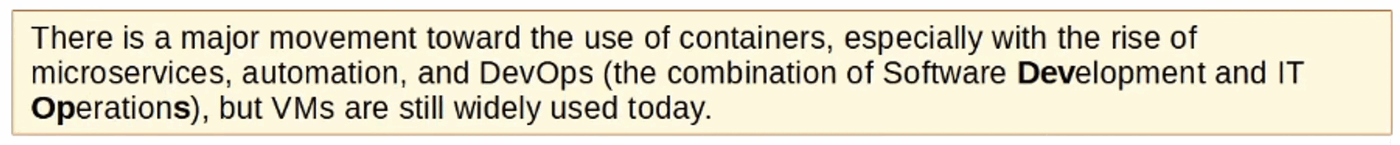
\includegraphics[keepaspectratio,alt={image}]{images/56-virtualization-containers/img-007.png}}
\end{figure}
